% !TeX root = d1.tex

\documentclass{article}

\usepackage{xcolor}
\usepackage[margin=0.5in]{geometry} 
\usepackage{graphicx}
\title{MindMerge --- Deliverable e 1}
\author{Gabriele Benetti, Gioele Berdardini, Luca Fossa Crescini, Luca Sartore}

\begin{document}
\maketitle


\tableofcontents

\section{SWAT Analysis}
\subsection{Strengths}
\begin{itemize}
    \item \textbf{Operating in an market that is hyped and growing: }
          The Artificial intelligence and LLM (large language models) market is currently on everyone's mouth.
          and is growing fast\dots this would make it easy for our team to find sell the product, and potentially find investors

    \item \textbf{The workplace is getting more and more digital: }
          In the last decades more and more jobs are getting used to using

    \item \textbf{: }
    \item \textbf{: }


\end{itemize}
\subsection{Weaknesses}

\subsection{Opportunities}

\subsection{Threads}

\section{Functional Requirements}
\begin{itemize}
    \item The system must allow owners for the creation of an Organization
    \item The system must allow Organizations for assigning tasks for their assignees
    \item Each task should be capable of having multiple subtasks in a tree structure
    \item Each task must have at least one manager
    \item Each task must have at least one assignee
    \item Each task should have a priority option
    \item Each task should have a deadline option
    \item Each task should have a state attribute
    \item Each task should have a manually managed notes section
    \item The system must allow users to be added to groups
    \item Each task must implement a permission system
    \item The permission system must implement various visibility and modification options
    \item The system must enforce task permissions to each user
    \item The application must provide a manual report option
    \item The manual reports must be done by users
    \item The application must provide an automatic report option
    \item The automatic reports must be based off of user notes and reports
    \item The automatic reports must be created by the systemrichiedere chiarimento
    \item The system must use LLM systems for the creation of automatic reports
    \item The system must allow managers to request reports manually
    \item The system must allow managers to request reports automatically
    \item Managers must be able to set and edit the automatic reports request frequency
    \item The system must implement a Notification system
    \item The notification system must be available by both assignees and managers
    \item The notification system must show report requests issued by managers
    \item The notification system must show task completition pings to each appropriate member of a task
    \item The notification system must show help and clarification messages issued by assignees
    \item The system must allow its users the option for enabling the notification
    \item The system must allow its users the option for disabling the notification
\end{itemize}

\section{Non-functional Requirements}
\subsection{Performance}
\begin{itemize}
    \item The software should implement tools for performance monitoring
    \item The automatic report generation should take at most 3 seconds for each level of the task tree
    \item Notifications should be sent in less than 5 minutes from the happening of the triggering event
\end{itemize}

\subsection{Reliability}
\begin{itemize}
    \item The system should have minimum downtime and at least 99\% uptime
    \item The system should implement a way to avoid collisions if two or more users try to edit the same task simultaneously
    \item The automatic report generation should implement a system to prevent chatbot hallucination
\end{itemize}

\subsection{Usability}
\begin{itemize}
    \item The software and the UI should be easy to understand and friendly to use
    \item The automatically generated report should be as accurate as possible
\end{itemize}

\subsection{Scalability}
\begin{itemize}
    \item The system should be able to manage at least 100.000 users simultaneously
    \item The system should be able to manage at least 10.000.000 non-simultaneous users
    \item The system should be able to manage a task tree with at least 1000 tasks
    \item The system should be able to manage a task tree with an height of at least 10 levels
\end{itemize}

\subsection{Security}
\begin{itemize}
    \item The system should allow users to see and edit only tasks they are entitled to use
    \item Authentication procedure should rely on string encryption mechanisms
    \item The password recovery system should not compromise security
    \item A company's data should be encrypted in the database in order to avoid data leak in case of security breaches
\end{itemize}

\section{Use Case Diagram}
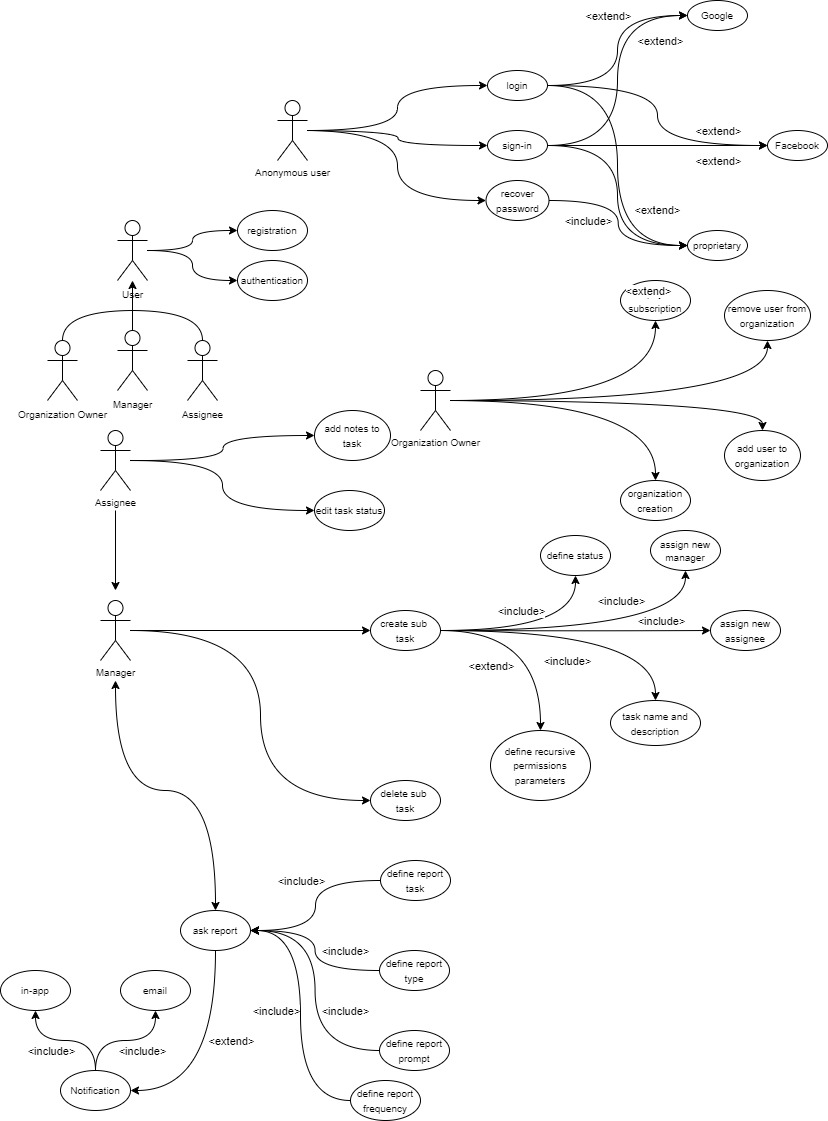
\includegraphics[width=\textwidth,height=\textheight,keepaspectratio]{images/UseCaseDiagram.jpg}

\section{Context Diagram}
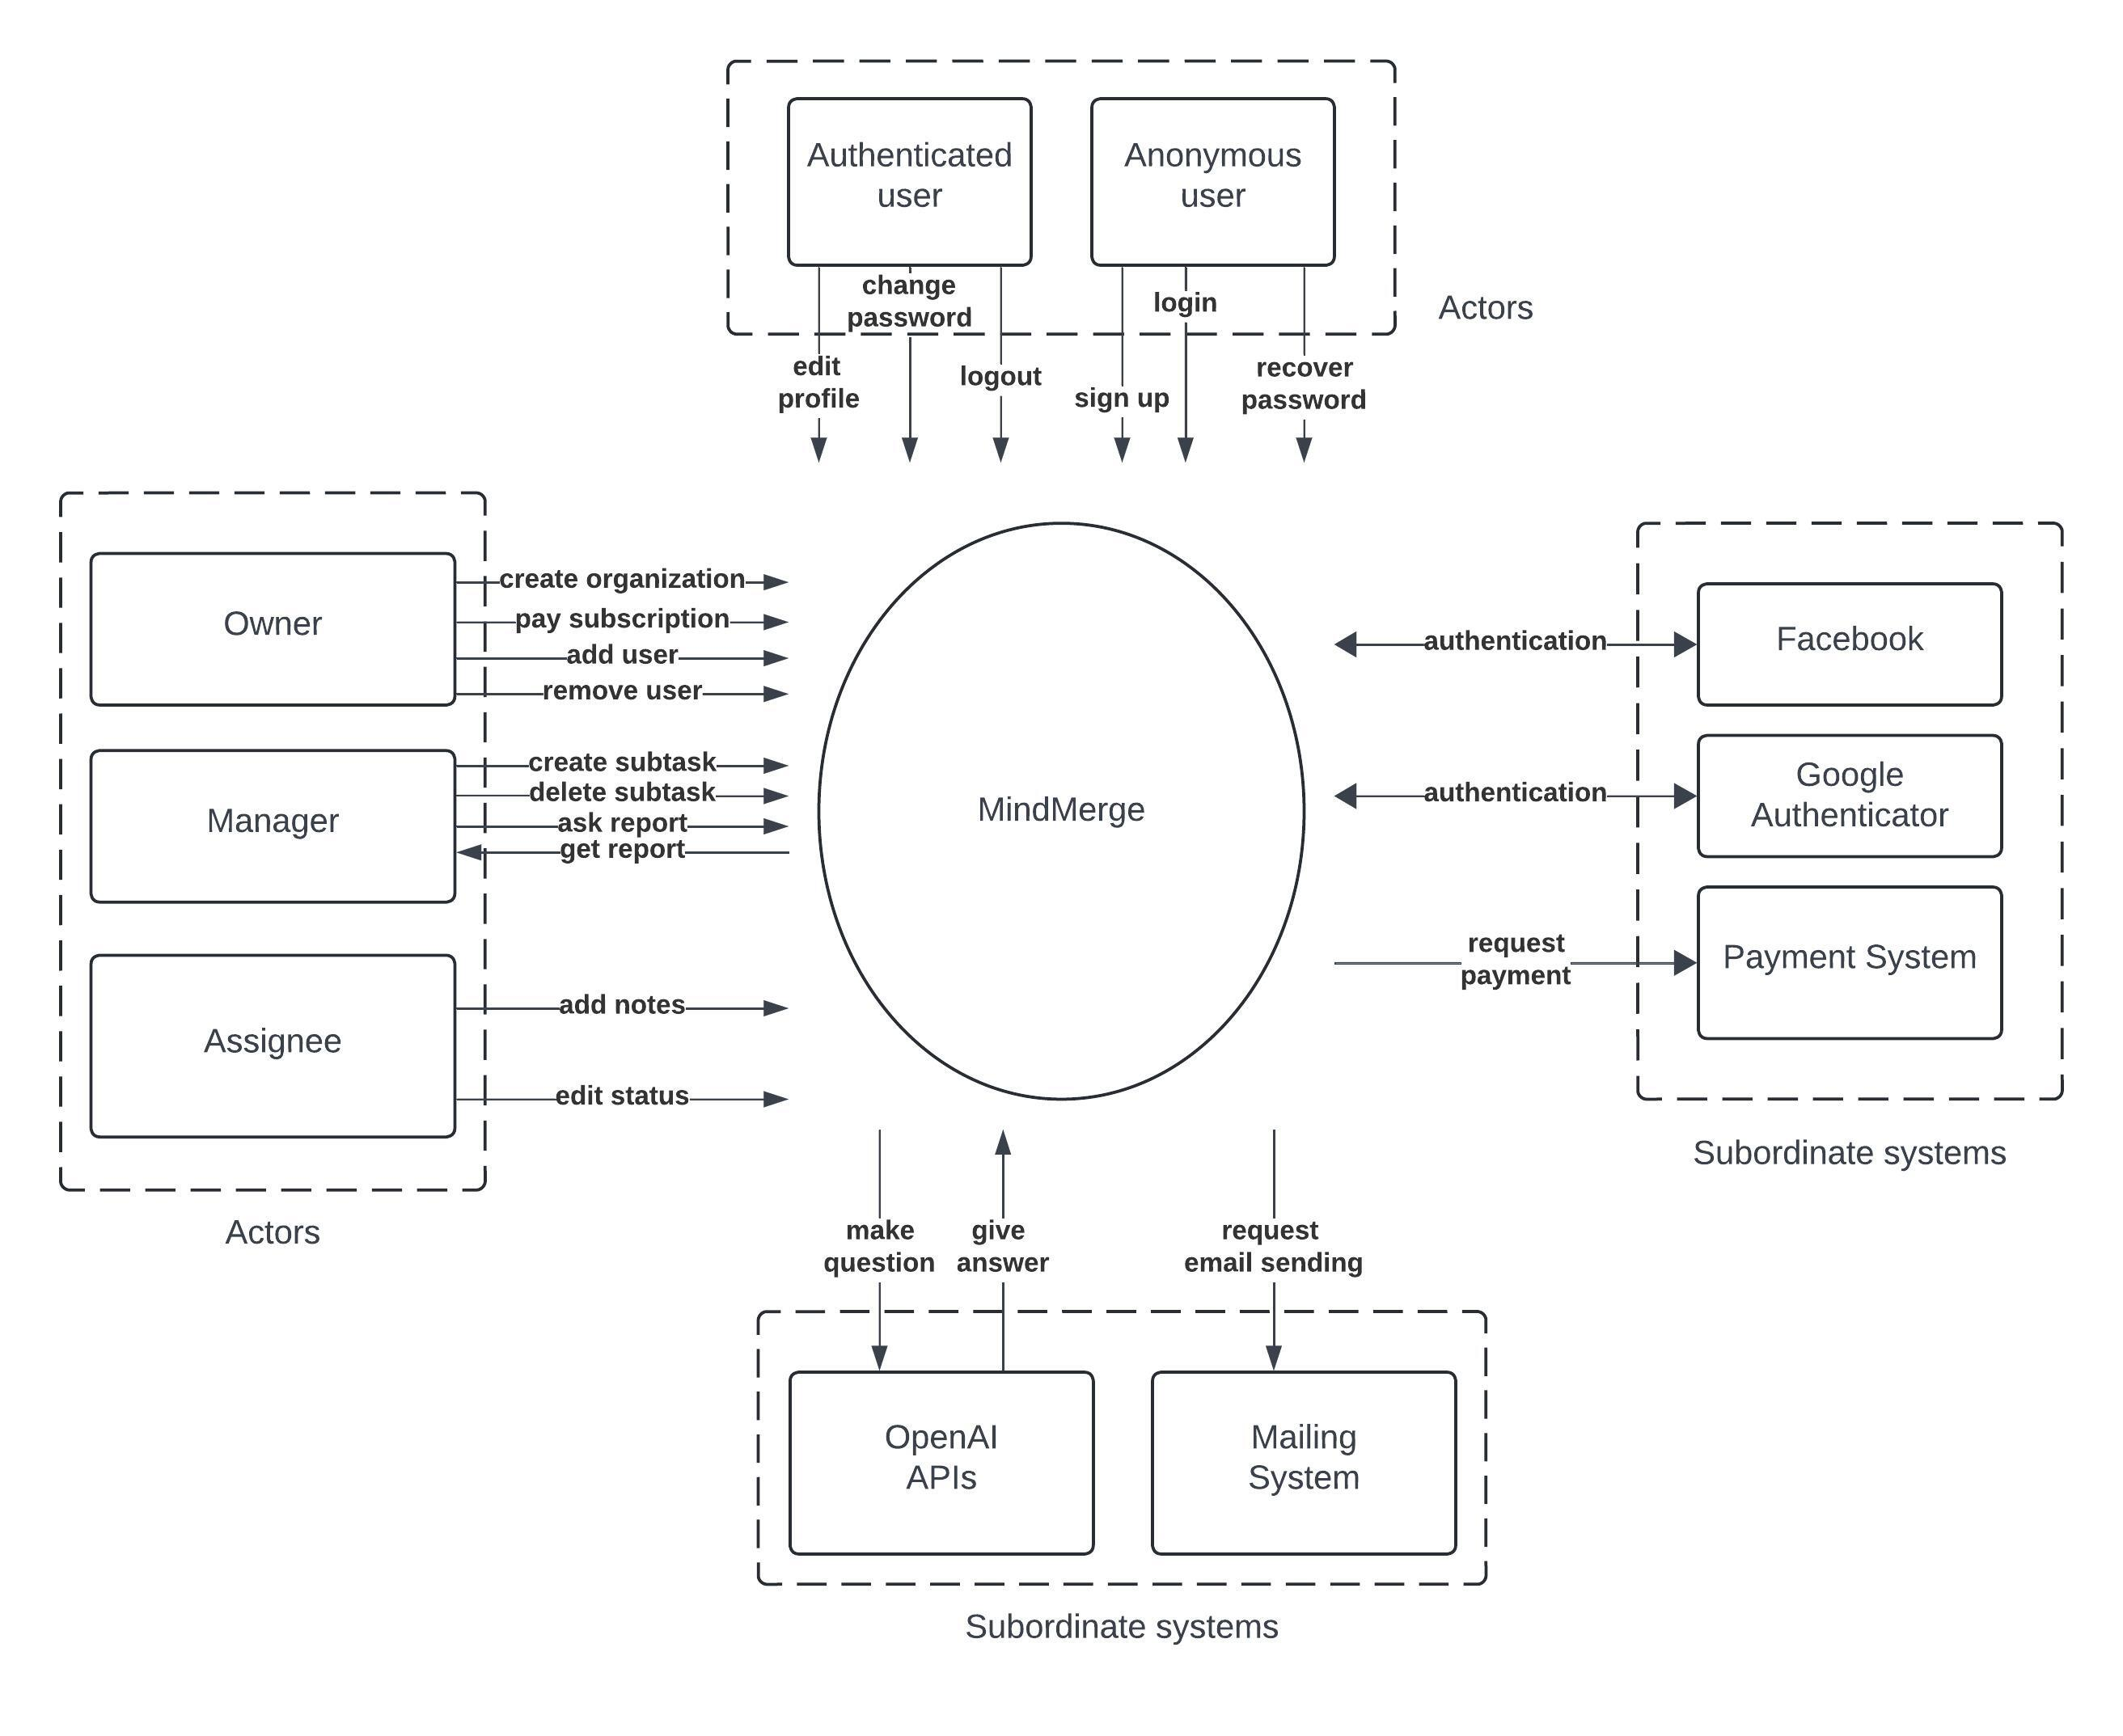
\includegraphics[width=\textwidth, height=\textheight, keepaspectratio]{images/context_diagram.jpeg}

\section{Components Diagram}

This section illustrate the component diagram of the system. To improve readability we split the components into several sub
components.
Each sub component has a color assigned to it, and the interfaces that are provided by that specific component are painted with the same color.
This helps to quickly identify which component is responsible for a specific interface.
\newline \newline
The list of sub components is the following:
\begin{itemize}
    \item \textcolor[HTML]{8CC86E}{\textbf{Data Base Manager: }} This component is responsible for managing the data base, it is an interface between
          the data base and the rest of the subsystems. The color assigned to this component is \textcolor[HTML]{8CC86E}{green}.
    \item \textcolor[HTML]{F0C832}{\textbf{Notification Manager: }} This component is responsible for managing the notifications;
          This means sending notification, and serve the data to the front end to visualize the pending notification of a user. The color assigned to this component is \textcolor[HTML]{F0C832}{yellow}.
    \item \textcolor[HTML]{FF0000}{\textbf{Account Manager: }} This component manage accounts, in particular it handles sign in, log in, account changes and account deletion.
          The color assigned to this component is \textcolor[HTML]{FF0000}{red}.
    \item \textcolor[HTML]{64C8BE}{\textbf{LLM Prompter: }} This component is a simple library that provide an interface to prompt different LLMs. It's objective is to make the
          implementation of the rest of the system agnostic from the specific LLM used. The color assigned to this component is \textcolor[HTML]{64C8BE}{aqua green}.
    \item \textcolor[HTML]{A0C8F0}{\textbf{Task Tree Navigator: }} This component is a simple library with some algorithm to navigate a tree data structure.
          In our specific case the tree represent the tasks and subtasks of an organization. Since this algorithms are used many
          times throughout the system they have been put in a specific component to make them reusable. The color assigned to this component is \textcolor[HTML]{A0C8F0}{light blue}.
    \item \textcolor[HTML]{FA9646}{\textbf{Report Manager: }} This component manage the reports, in particular it is responsible for generating report automatically (using an LLM) or manually (reminding users with a notification that they have to deliver a report).
          The component also allow users to set report schedule, so that the reports generation can be triggered automatically with a customizable frequency.
          The color assigned to this component is \textcolor[HTML]{FA9646}{orange}.
    \item \textcolor[HTML]{FF00FF}{\textbf{Organization Manager: }} This component allow an user to create an organization, or perform some action on his organizations,
          like adding/removing a user, or paying the subscription to use the software. The color assigned to this component is \textcolor[HTML]{FF00FF}{purple}.
    \item \textcolor[HTML]{2682D5}{\textbf{Task Manager: }} This component allow users to interact with the tasks.
          In particular it is responsible to visualize, create, delete and edit tasks inside one organization. The color assigned to this component is \textcolor[HTML]{2682D5}{blue}.
    \item \textbf{Front End: } This component is responsible for the visualization of the data, and the interaction with the user. This component dose not have a specific color assigned to it, since it dose not provide any interface to other components.
    \item \textcolor[HTML]{E68CB4}{\textbf{External APIs: }} All interfaces provided by external APIs in the system (like authentication, payment, etc.) are painted with the color \textcolor[HTML]{E68CB4}{pink}.
\end{itemize}

\subsection{Data Base Manager}
\subsubsection{Diagram}
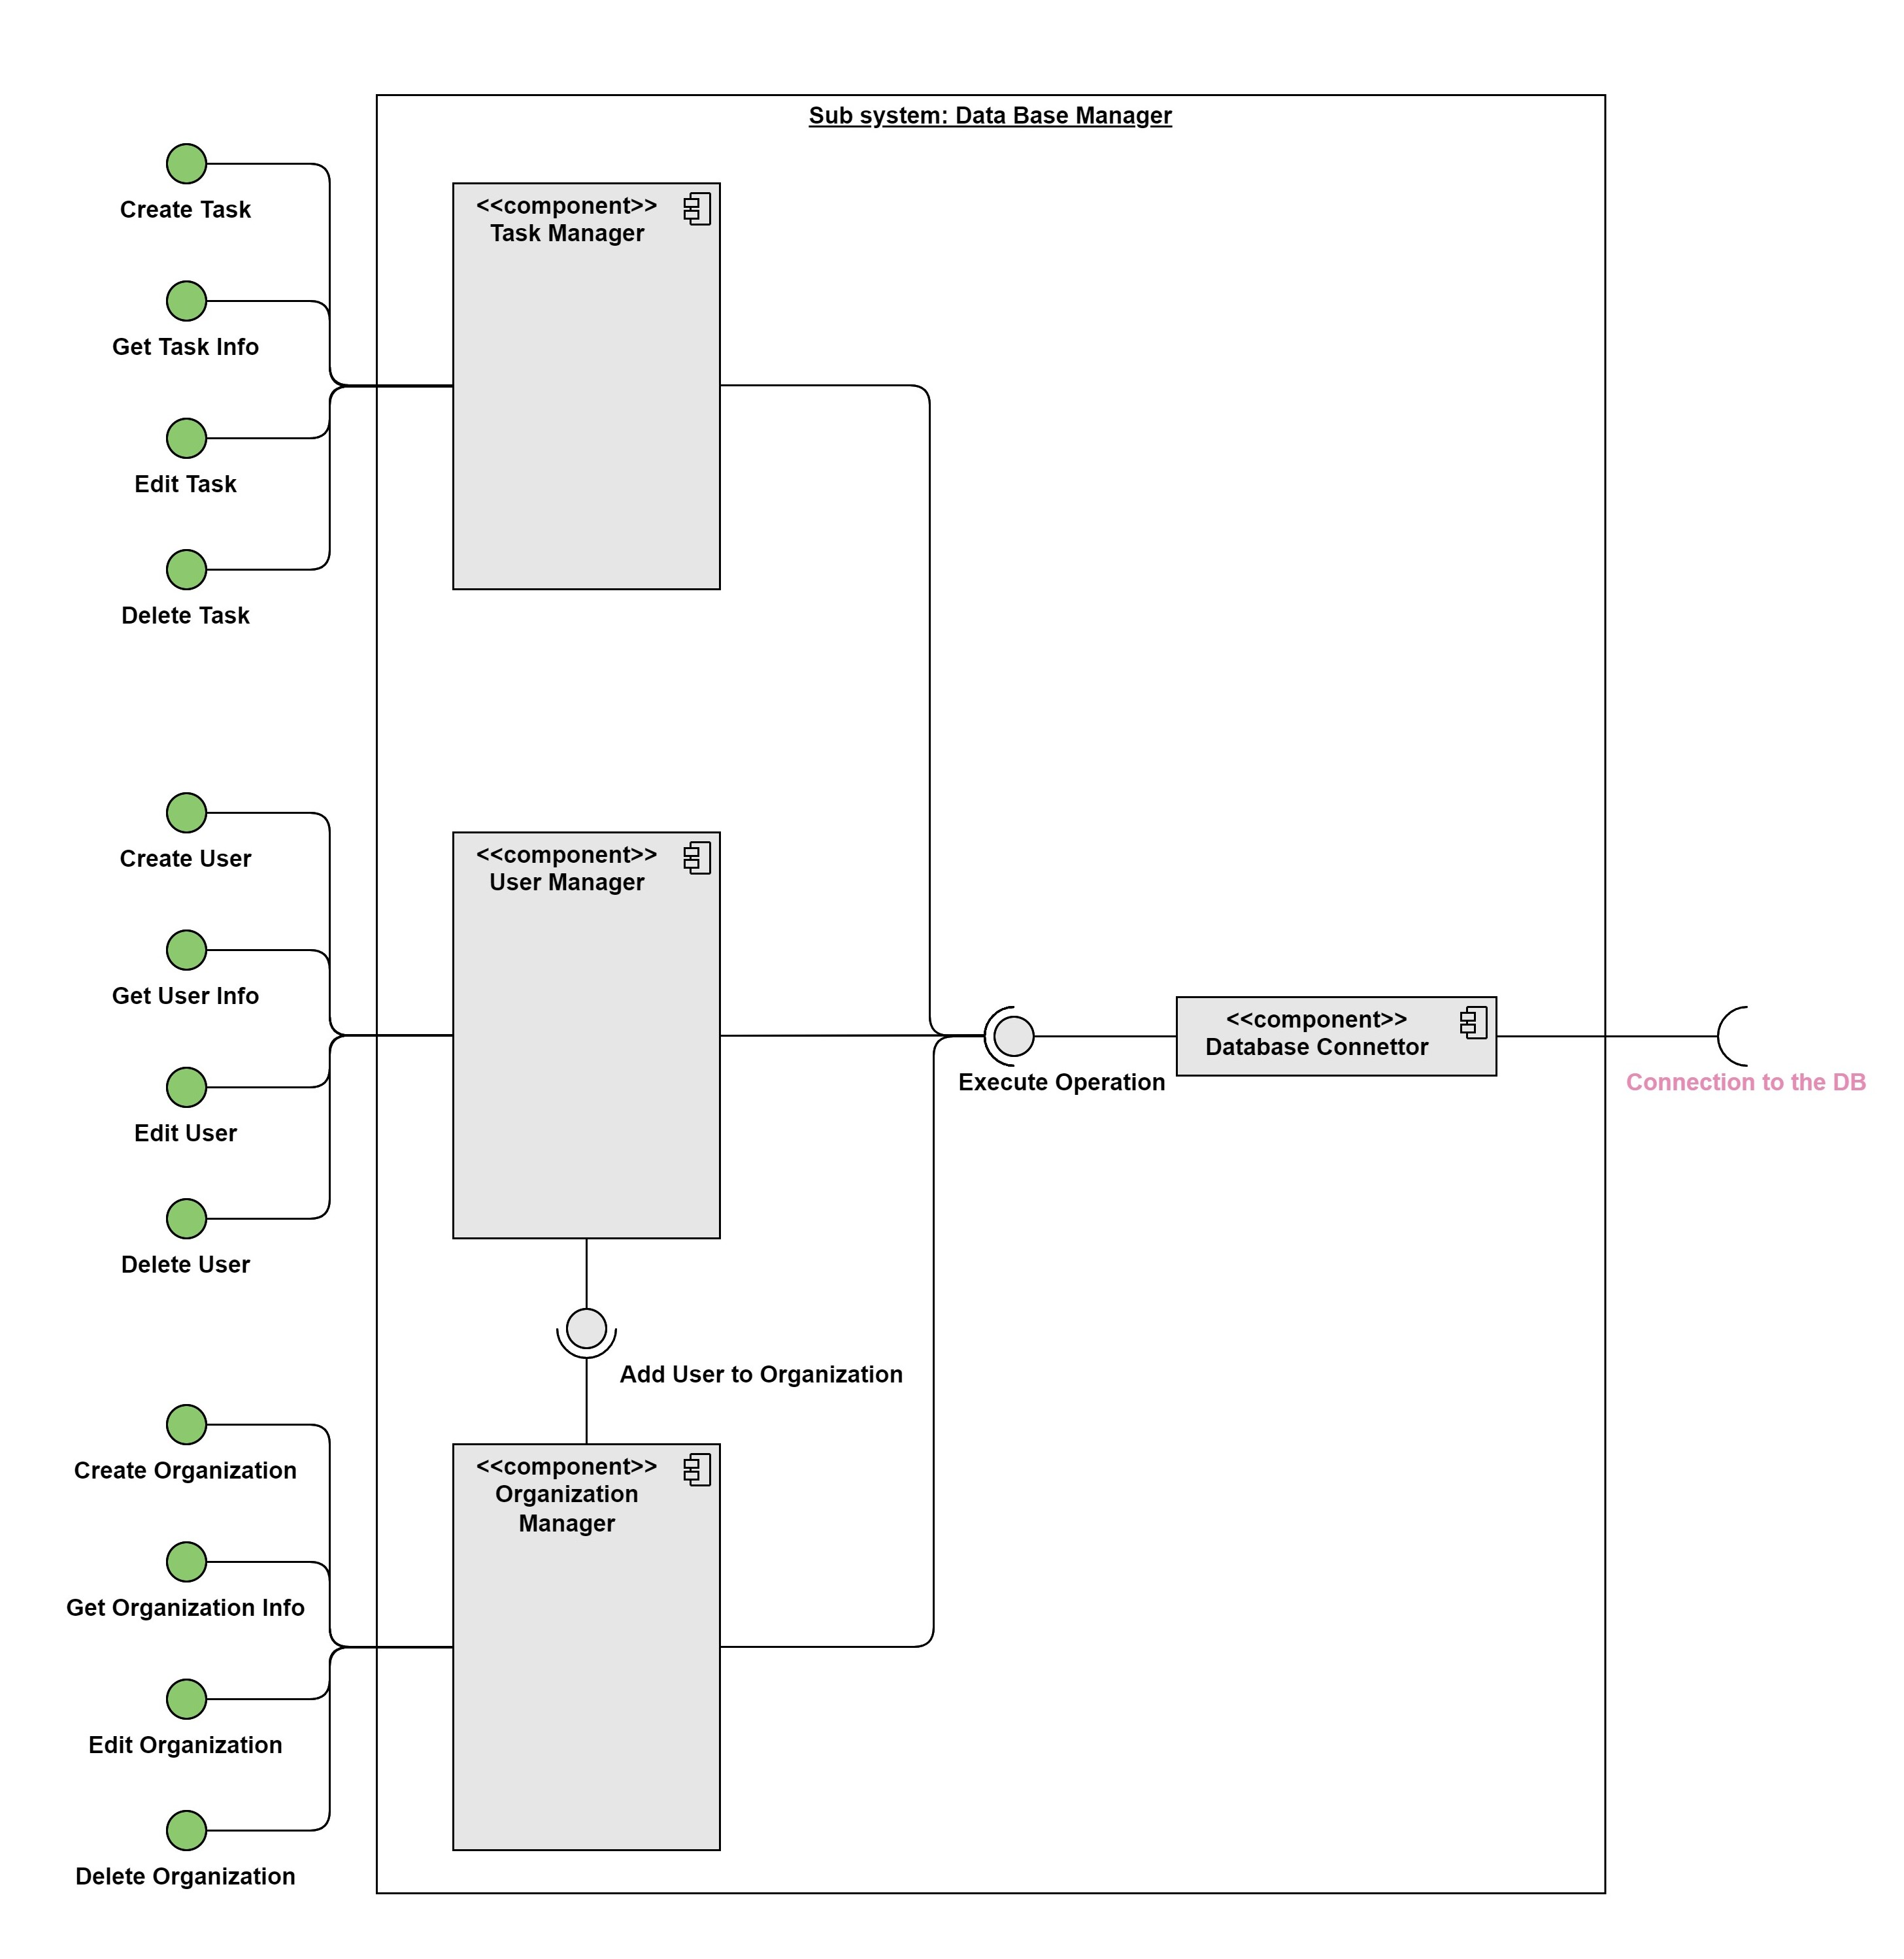
\includegraphics[width=\textwidth,height=\textheight,keepaspectratio]{images/component_diagram/data_base_manager.jpg}
\subsubsection{Descriptions}

We have model the system with 3 particular objects (tasks, users and organizations).
The database manager has a specific component to manage each one of them. The interfaces provided
are divided fot the kind of action that needs to be performed (creation, deletion, modification or read operations).\newline
The ``Database Connector'' component is used to hide the all the specific and superfluous detail about connecting to a
database (like authentication, api version ecc.)

\subsection{Notification Manager}
\subsubsection{Diagram}
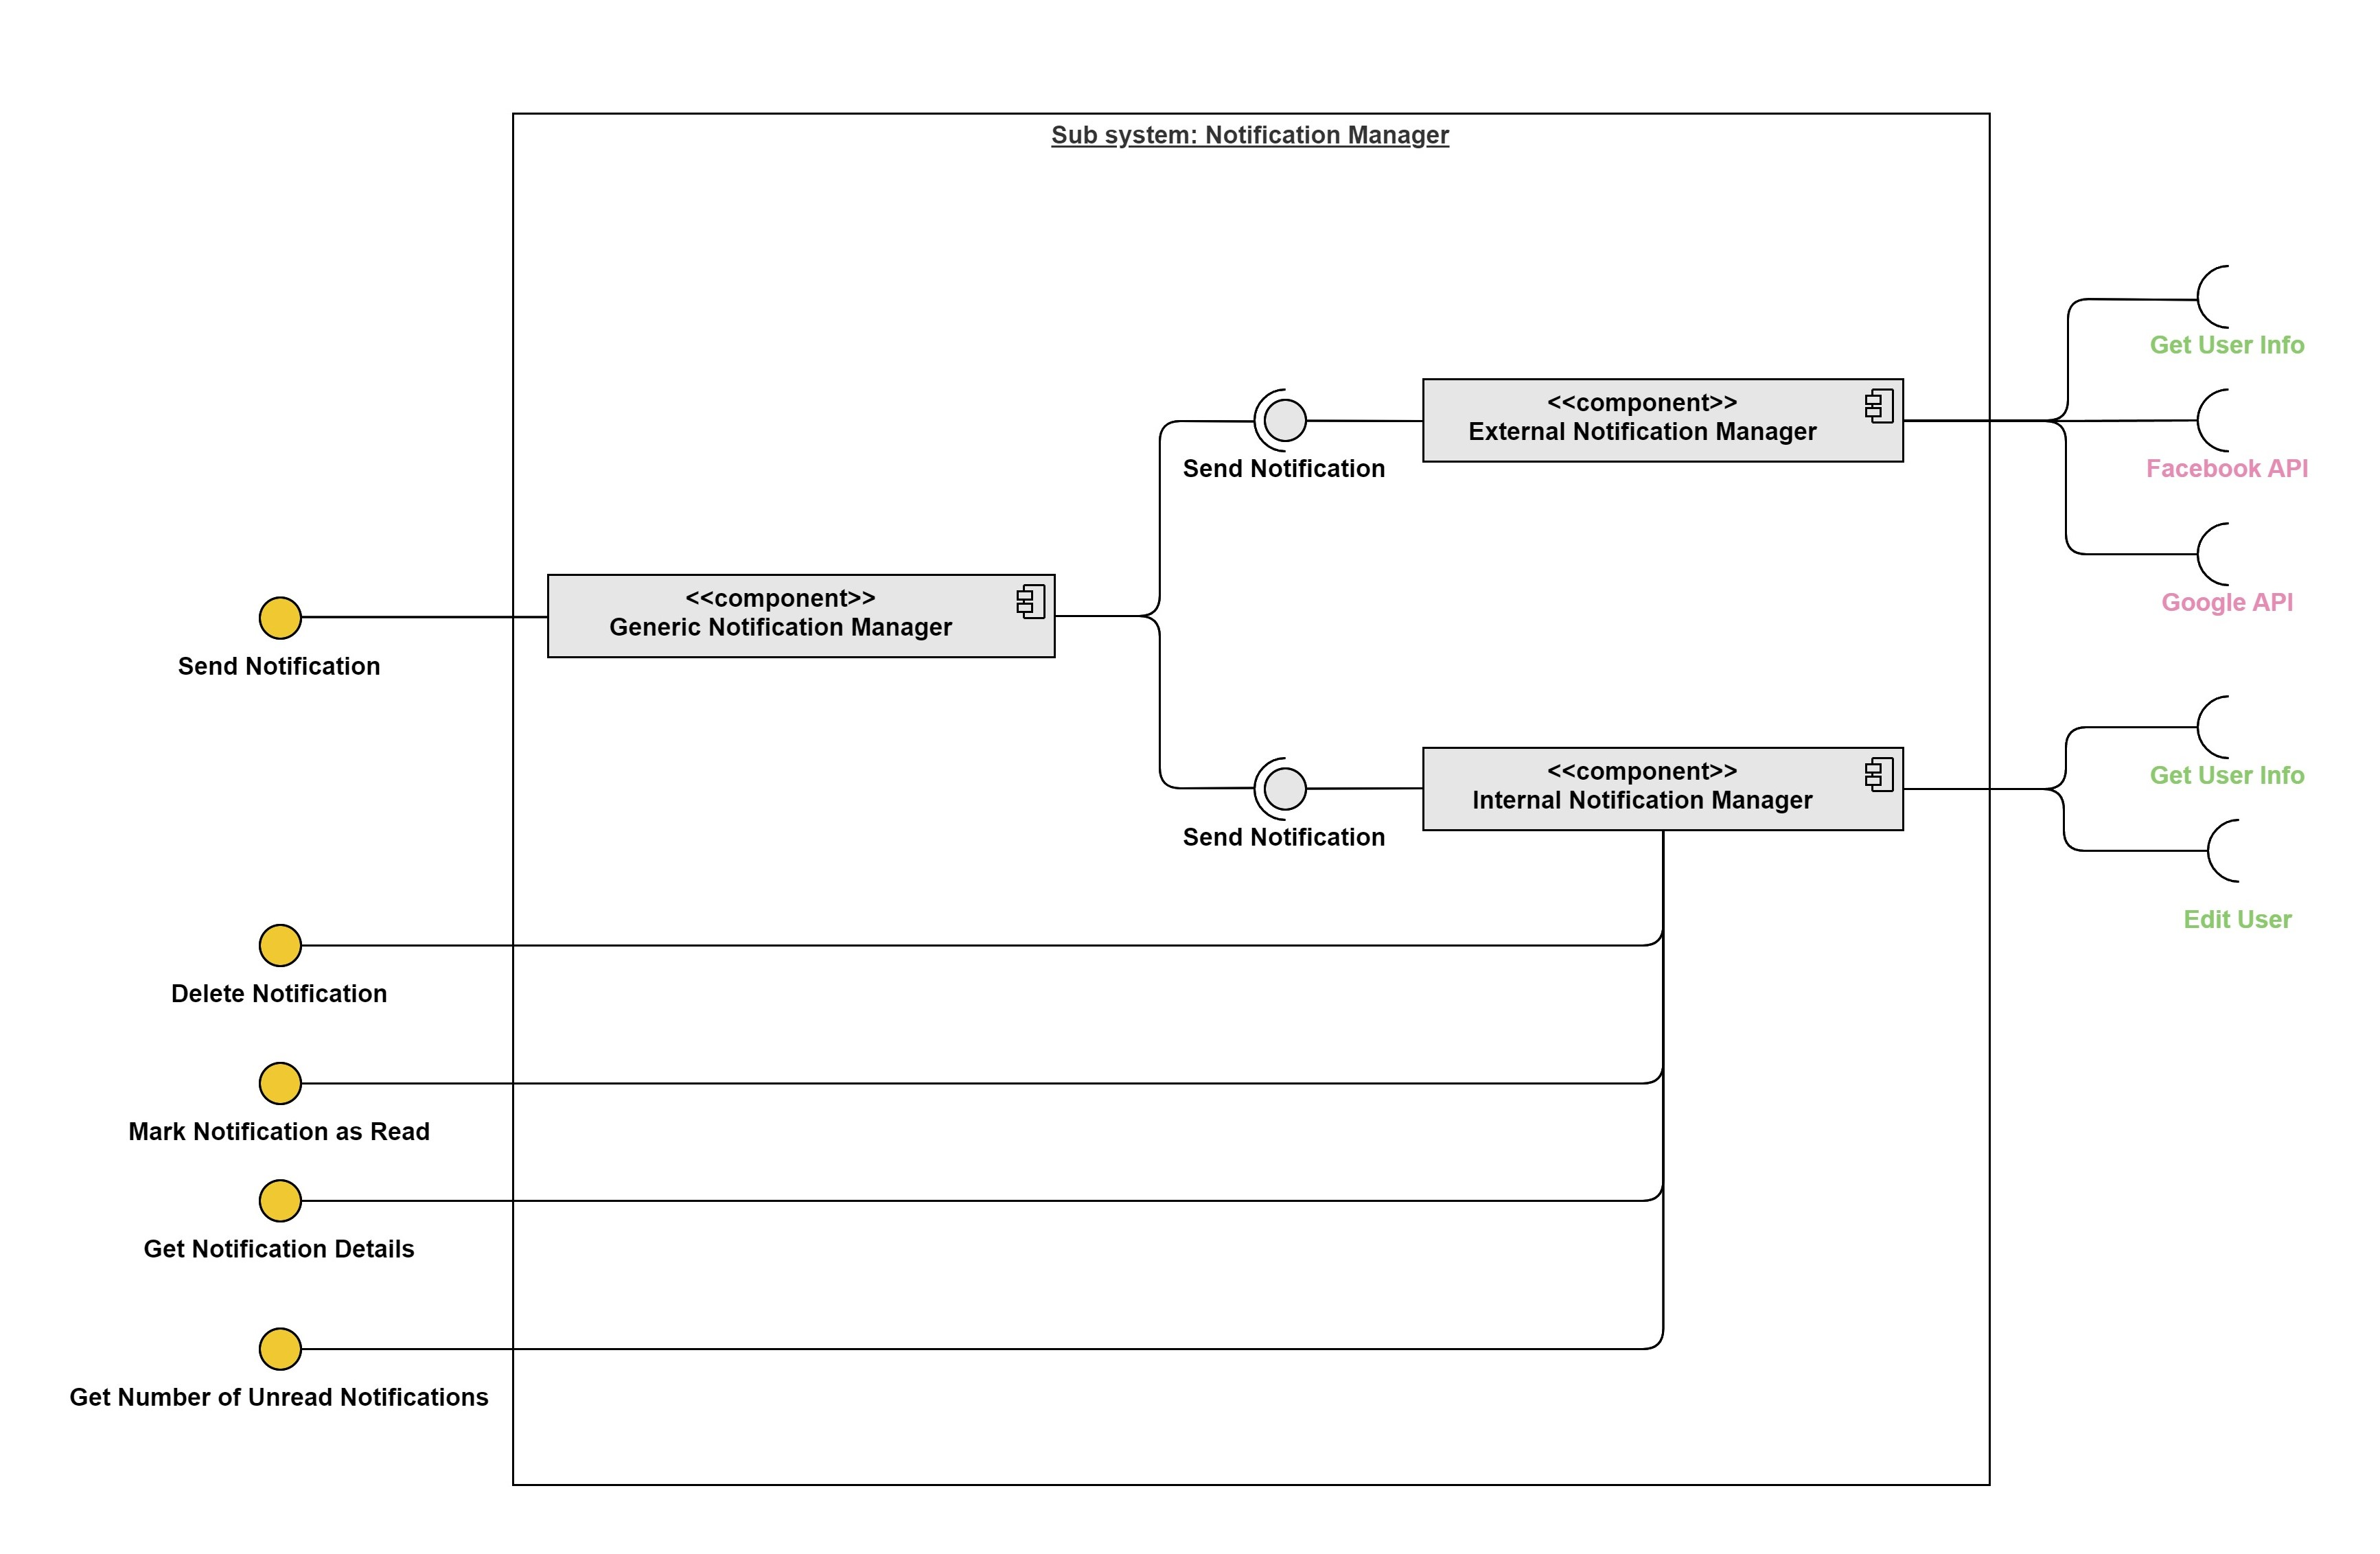
\includegraphics[width=\textwidth,height=\textheight,keepaspectratio]{images/component_diagram/notification_manager.jpg}
\subsubsection{Descriptions}
The notification manager system has 2 specific tasks:
\begin{itemize}
    \item Allowing other components to send notification to users.

          This is done by the ``send notification'' interface
    \item Allow a user to visualize pending notification in the front end

          This id done by the other 4 interfaces
\end{itemize}

The system is composed of 3 different component
\begin{itemize}
    \item \textbf{Generic Notification Manager: }

          This component is the one that provided the ``Send Notification'' interface, and it only act as
          a switch. The system allow for notification to be sent either via mail, or with an in-app notification.
          When a notification comes in to be send this component will decide where to send it.
    \item \textbf{External Notification Manager: }

          This component will send a mail with a notification to a specific user.
          This component has various external APIs connected to it, as how the notification is sent will depend on how the user signed In.
    \item \textbf{Internal Notification Manager: }

          This component manage the in-app notifications. It can either be asked to send a notification (in this case it writes it in the database)
          or it can be asked to get a notification by the front end, so that it can be visualized (in this case it reads the necessary data from the database)

\end{itemize}

\subsection{Account Manager}
\subsubsection{Diagram}
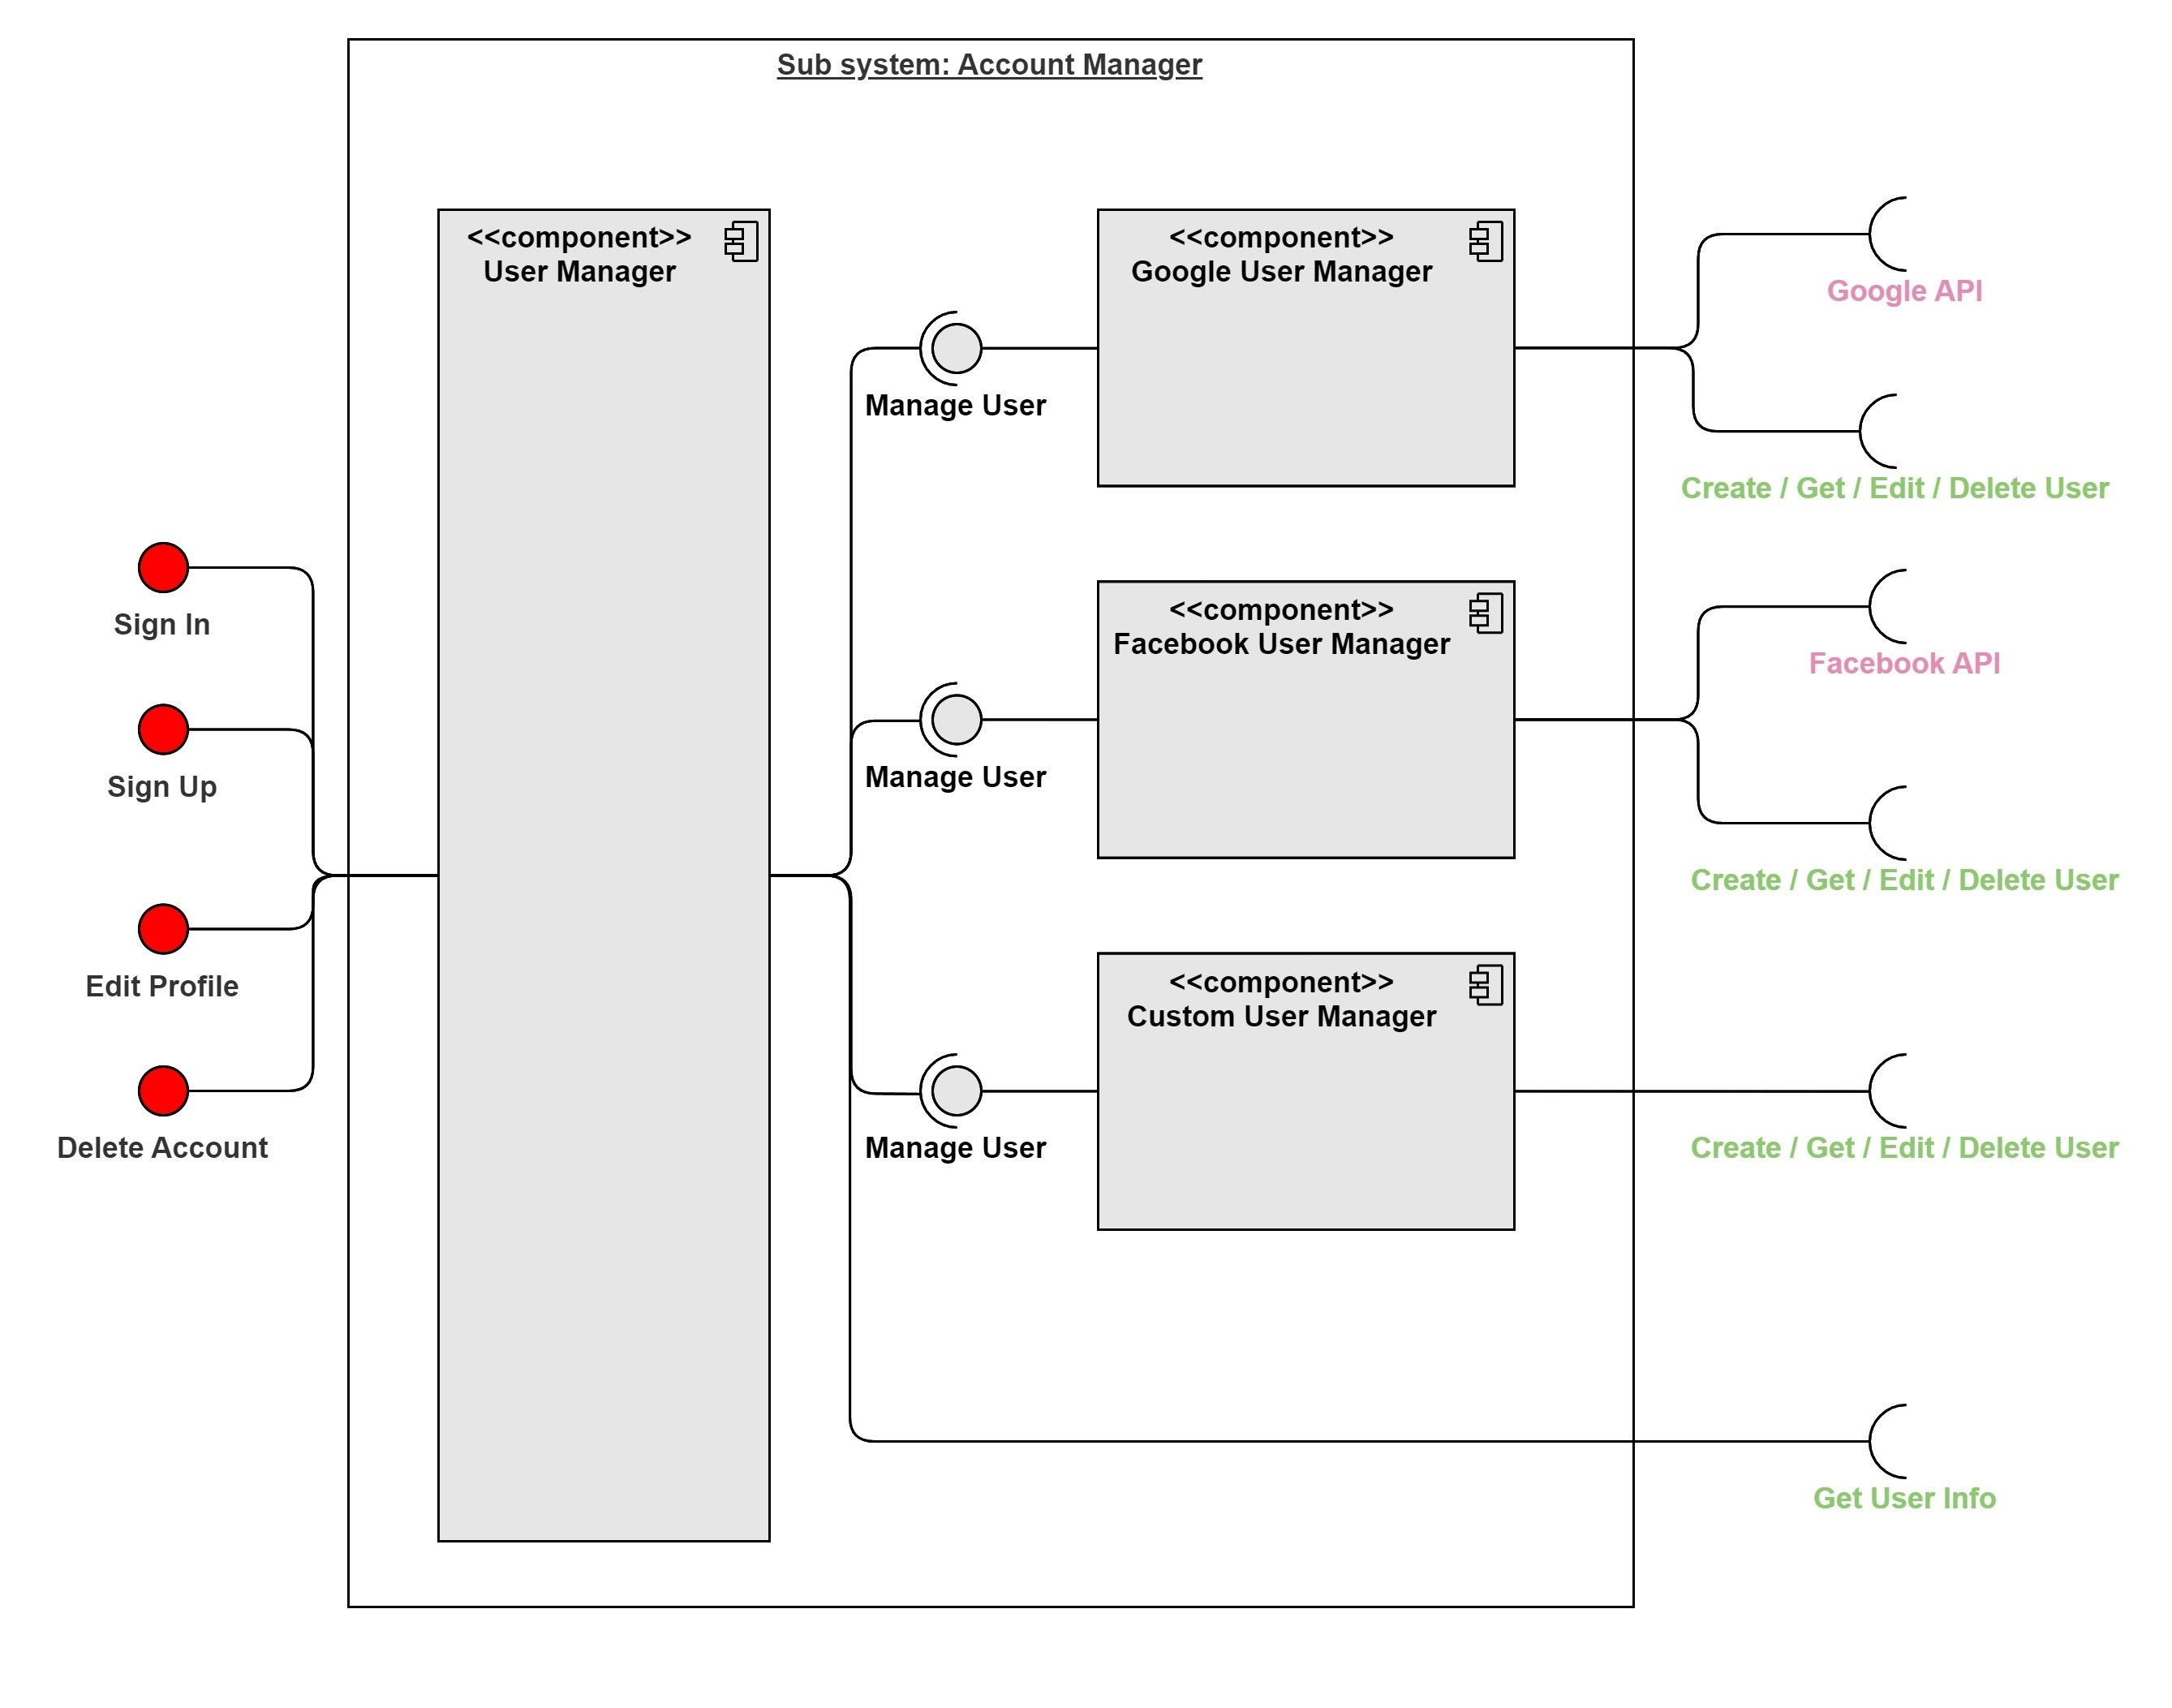
\includegraphics[width=\textwidth,height=\textheight,keepaspectratio]{images/component_diagram/account_manager.jpg}
\subsubsection{Descriptions}
The account manager system allow users to register, log in, delete account and change account information (like password, name, ecc.).

The specific implementation depends on how the user signed in. For this reason the system has a switch component (``User Manager'')
that will decide which specific implementation to use for each specific user. Once this is decided the user
can be handled by one of the 3 components:
\begin{itemize}
    \item \textbf{Google User Manager: }

          This component will handle all the user that signed in with a google account.
    \item \textbf{Facebook User Manager: }

          This component will handle all the user that signed in with a facebook account.
    \item \textbf{Custom User Manager: }

          This component will handle all the user that register with an email and password.
\end{itemize}
Note that we have bundled the database interfaces for managing users into one single interface to enhance readability.
\subsection{LLM Prompter}
\subsubsection{Diagram}
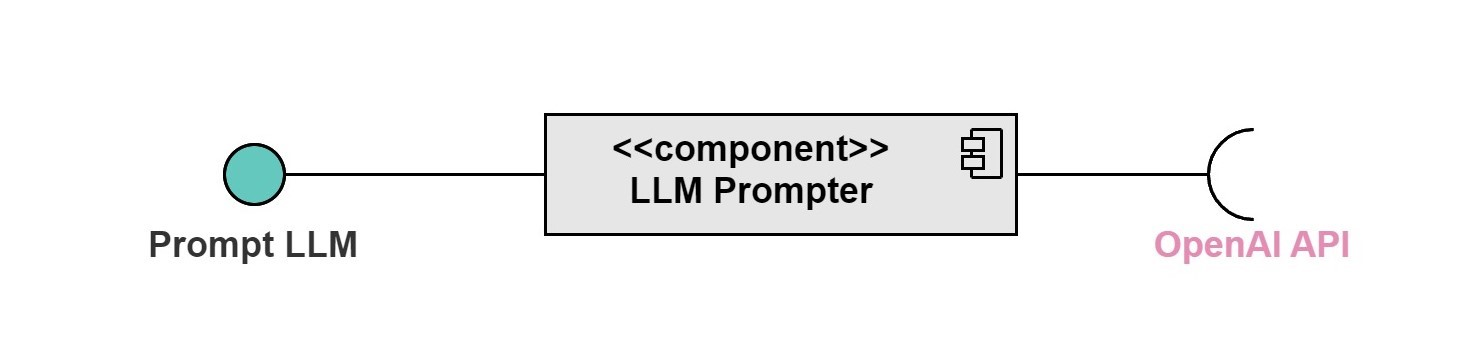
\includegraphics[width=\textwidth,height=\textheight,keepaspectratio]{images/component_diagram/llm_prompter.jpg}
\subsubsection{Descriptions}
This is a simple component that abstract the detail about the specific LLM that is been used from the rest of the system.
This is a good practice that can save some time in the future, if we decide to change the LLM that we are using.
In this example we are using Open AI APIs.

\subsection{Task Tree Navigator}
\subsubsection{Diagram}
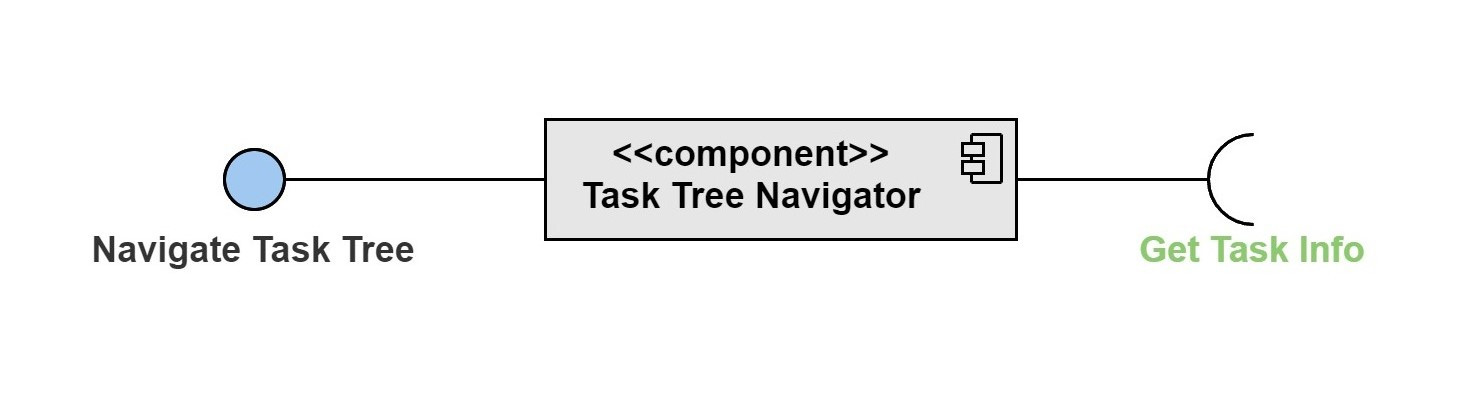
\includegraphics[width=\textwidth,height=\textheight,keepaspectratio]{images/component_diagram/task_tree_navigator.jpg}
\subsubsection{Descriptions}
This component provide some library useful to navigate the task tree. For example it can be used to find all the children of a task, up to a certain depth.

\subsection{Report Manager}
\subsubsection{Diagram}
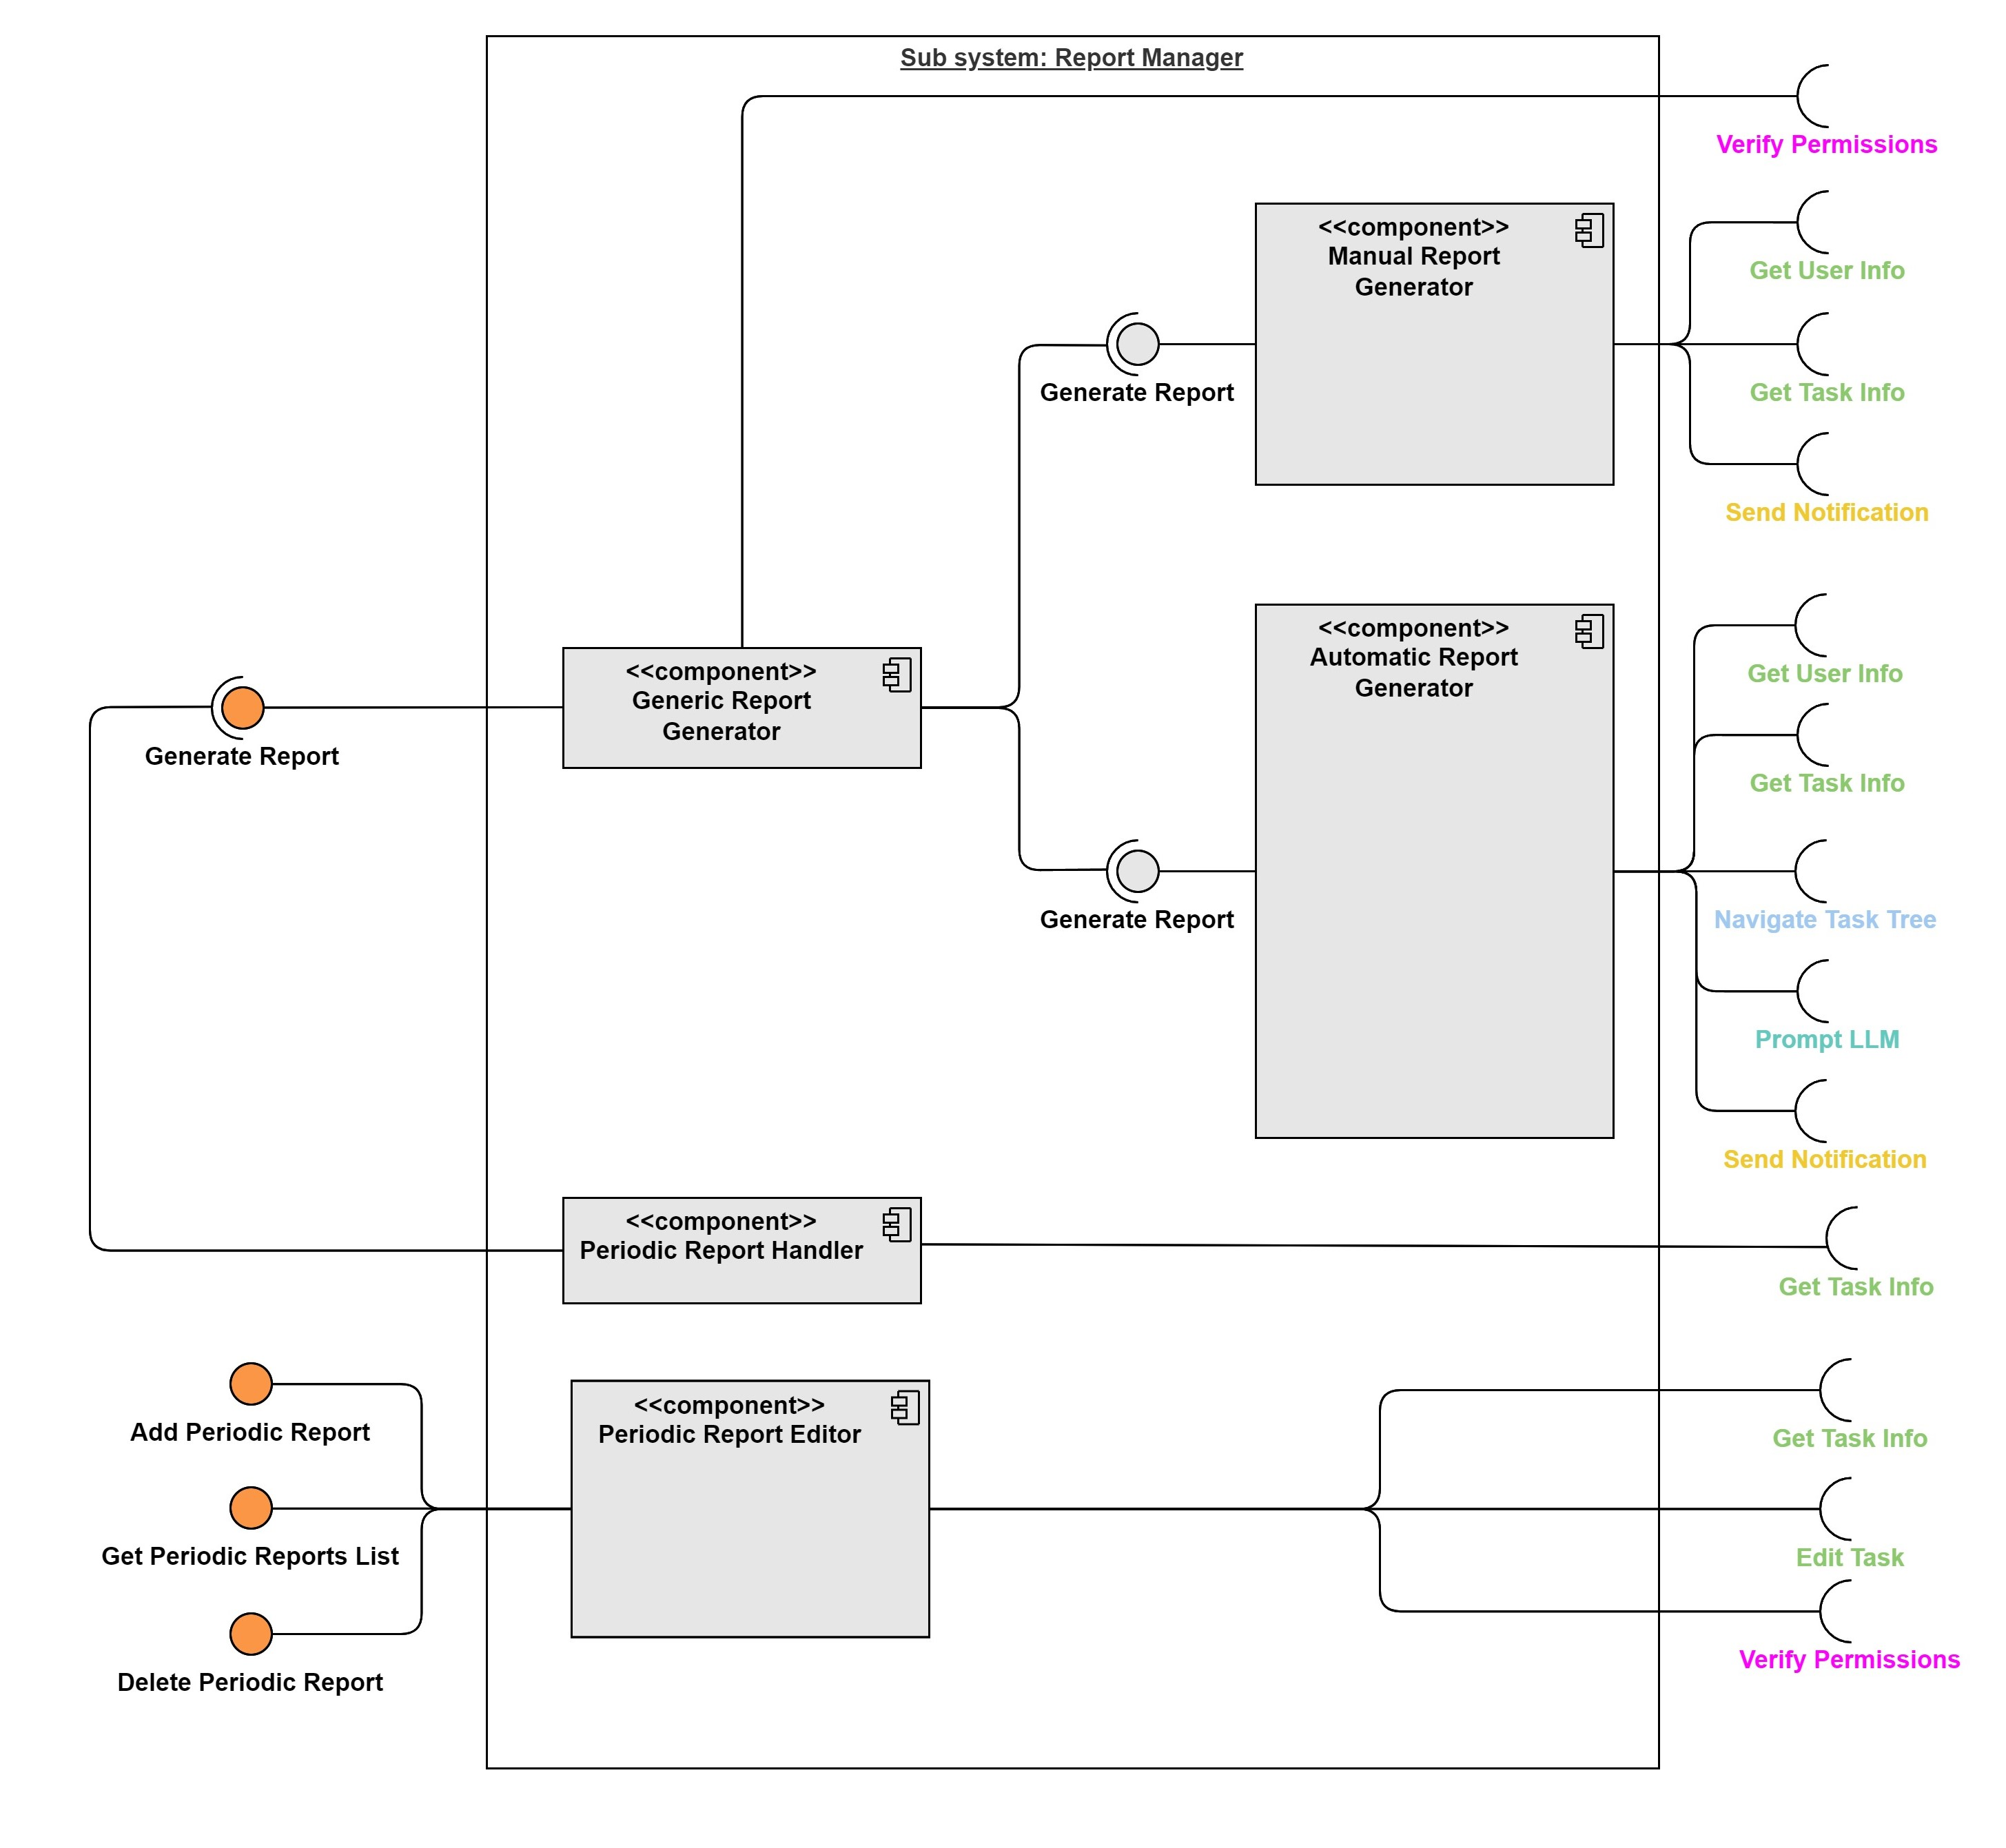
\includegraphics[width=\textwidth,height=\textheight,keepaspectratio]{images/component_diagram/report_manager.jpg}
\subsubsection{Descriptions}
The report manager have two main tasks:
\begin{itemize}
    \item Generating reports (both manually and automatically) 
    \item Managing the report schedule 
\end{itemize}

The system is composed of 5 different components:

\begin{itemize}
    \item \textbf{Manual Report Generator: }

    This component is responsible for generating manual reports. A manual report is a report that ir generated by a user, and not by the system.
    So in practice this component will just remind the user that he has to deliver a report.
    \item \textbf{Automatic Report Generator: }

    This component is responsible for generating automatic reports. An automatic report is a report that is generated ry the system,
    using an LLM. This component will use some LLM APIs, as well as the data that it could find in the database to generate the report, and then it will deliver It
    to the user how requested it, using the notification system.

    \item \textbf{Generic Report Generator: }
    
    This component is the one that provided the ``Generate Report'' interface, and it only act as a switch, That 
    will forward the request to the correct component (manual or automatic report generator).

    \item \textbf{Periodic Report Editor: }

    This component is responsible for managing the report schedule.
    It will allow users to set the frequency of the scheduled reports, as well as to edit or delete them.

    \item \textbf{Periodic Report Handler: }
    
    This component is responsible for handling the scheduled reports.
    It will read the schedule from the database, and then it will trigger a report generation event when the time comes.

\end{itemize}

\subsection{Task Manager}
\subsubsection{Diatgram}
\begin{center}
    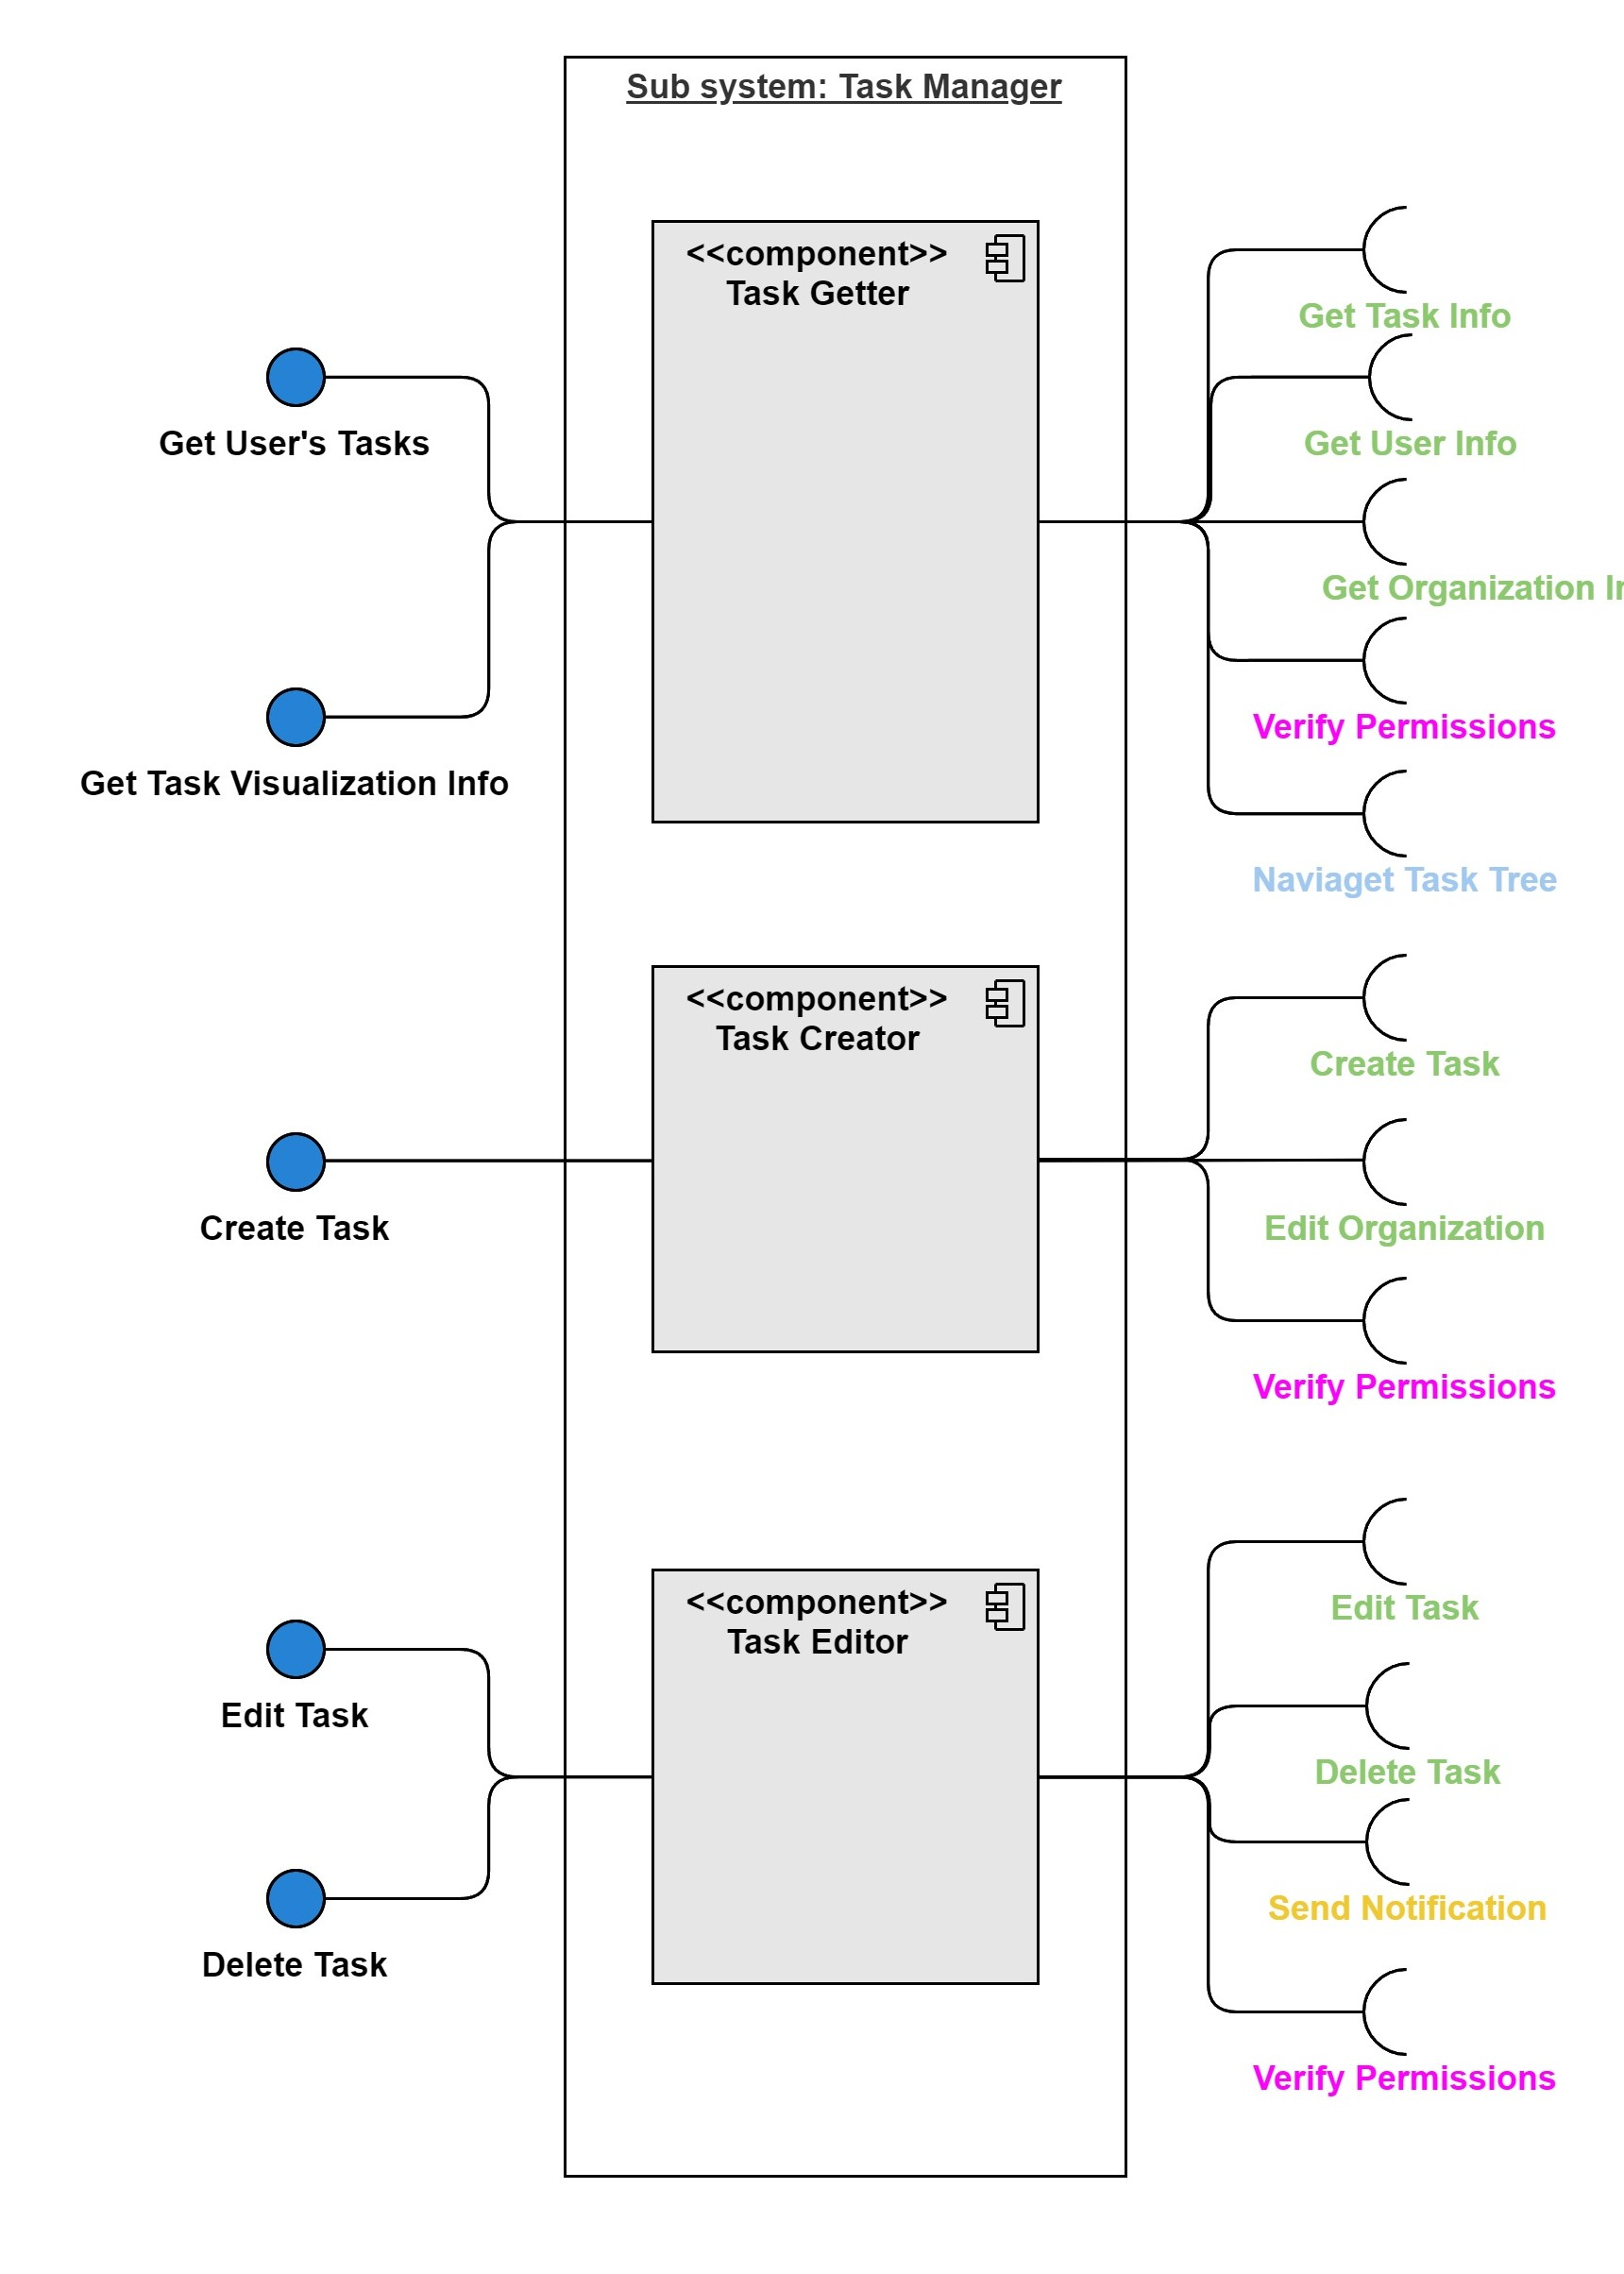
\includegraphics[width=5.5in,keepaspectratio]{images/component_diagram/task_manager.jpg}
\end{center}
\subsubsection{Descriptions}

The task manager is the component that allow users to interact with the tasks.
The interaction are divided in 3 main categories:
\begin{itemize}
    \item \textbf{Task Creation: }
    
    This is the process of creating a new task. That include operations like 
    setting the task name, the father task, the assignees, the managers ecc.
    This operations are handled by the ``Task Creator'' component.
    \item \textbf{Task Modification: }
    This is the process of modifying an existing task. That include operations like adding a descriptions or some notes,
    changing state, deadline assignee ecc; or even deleting the task.
    This operations are handled by the ``Task Editor'' component.
    \item \textbf{Task Reading Operation: }
    This process is responsible for reading the task data from the database, and then serve it to the front end.
    This operations are handled by the ``Task Getter'' component.
\end{itemize}

\subsection{Front End}
\subsubsection{Diatgram}
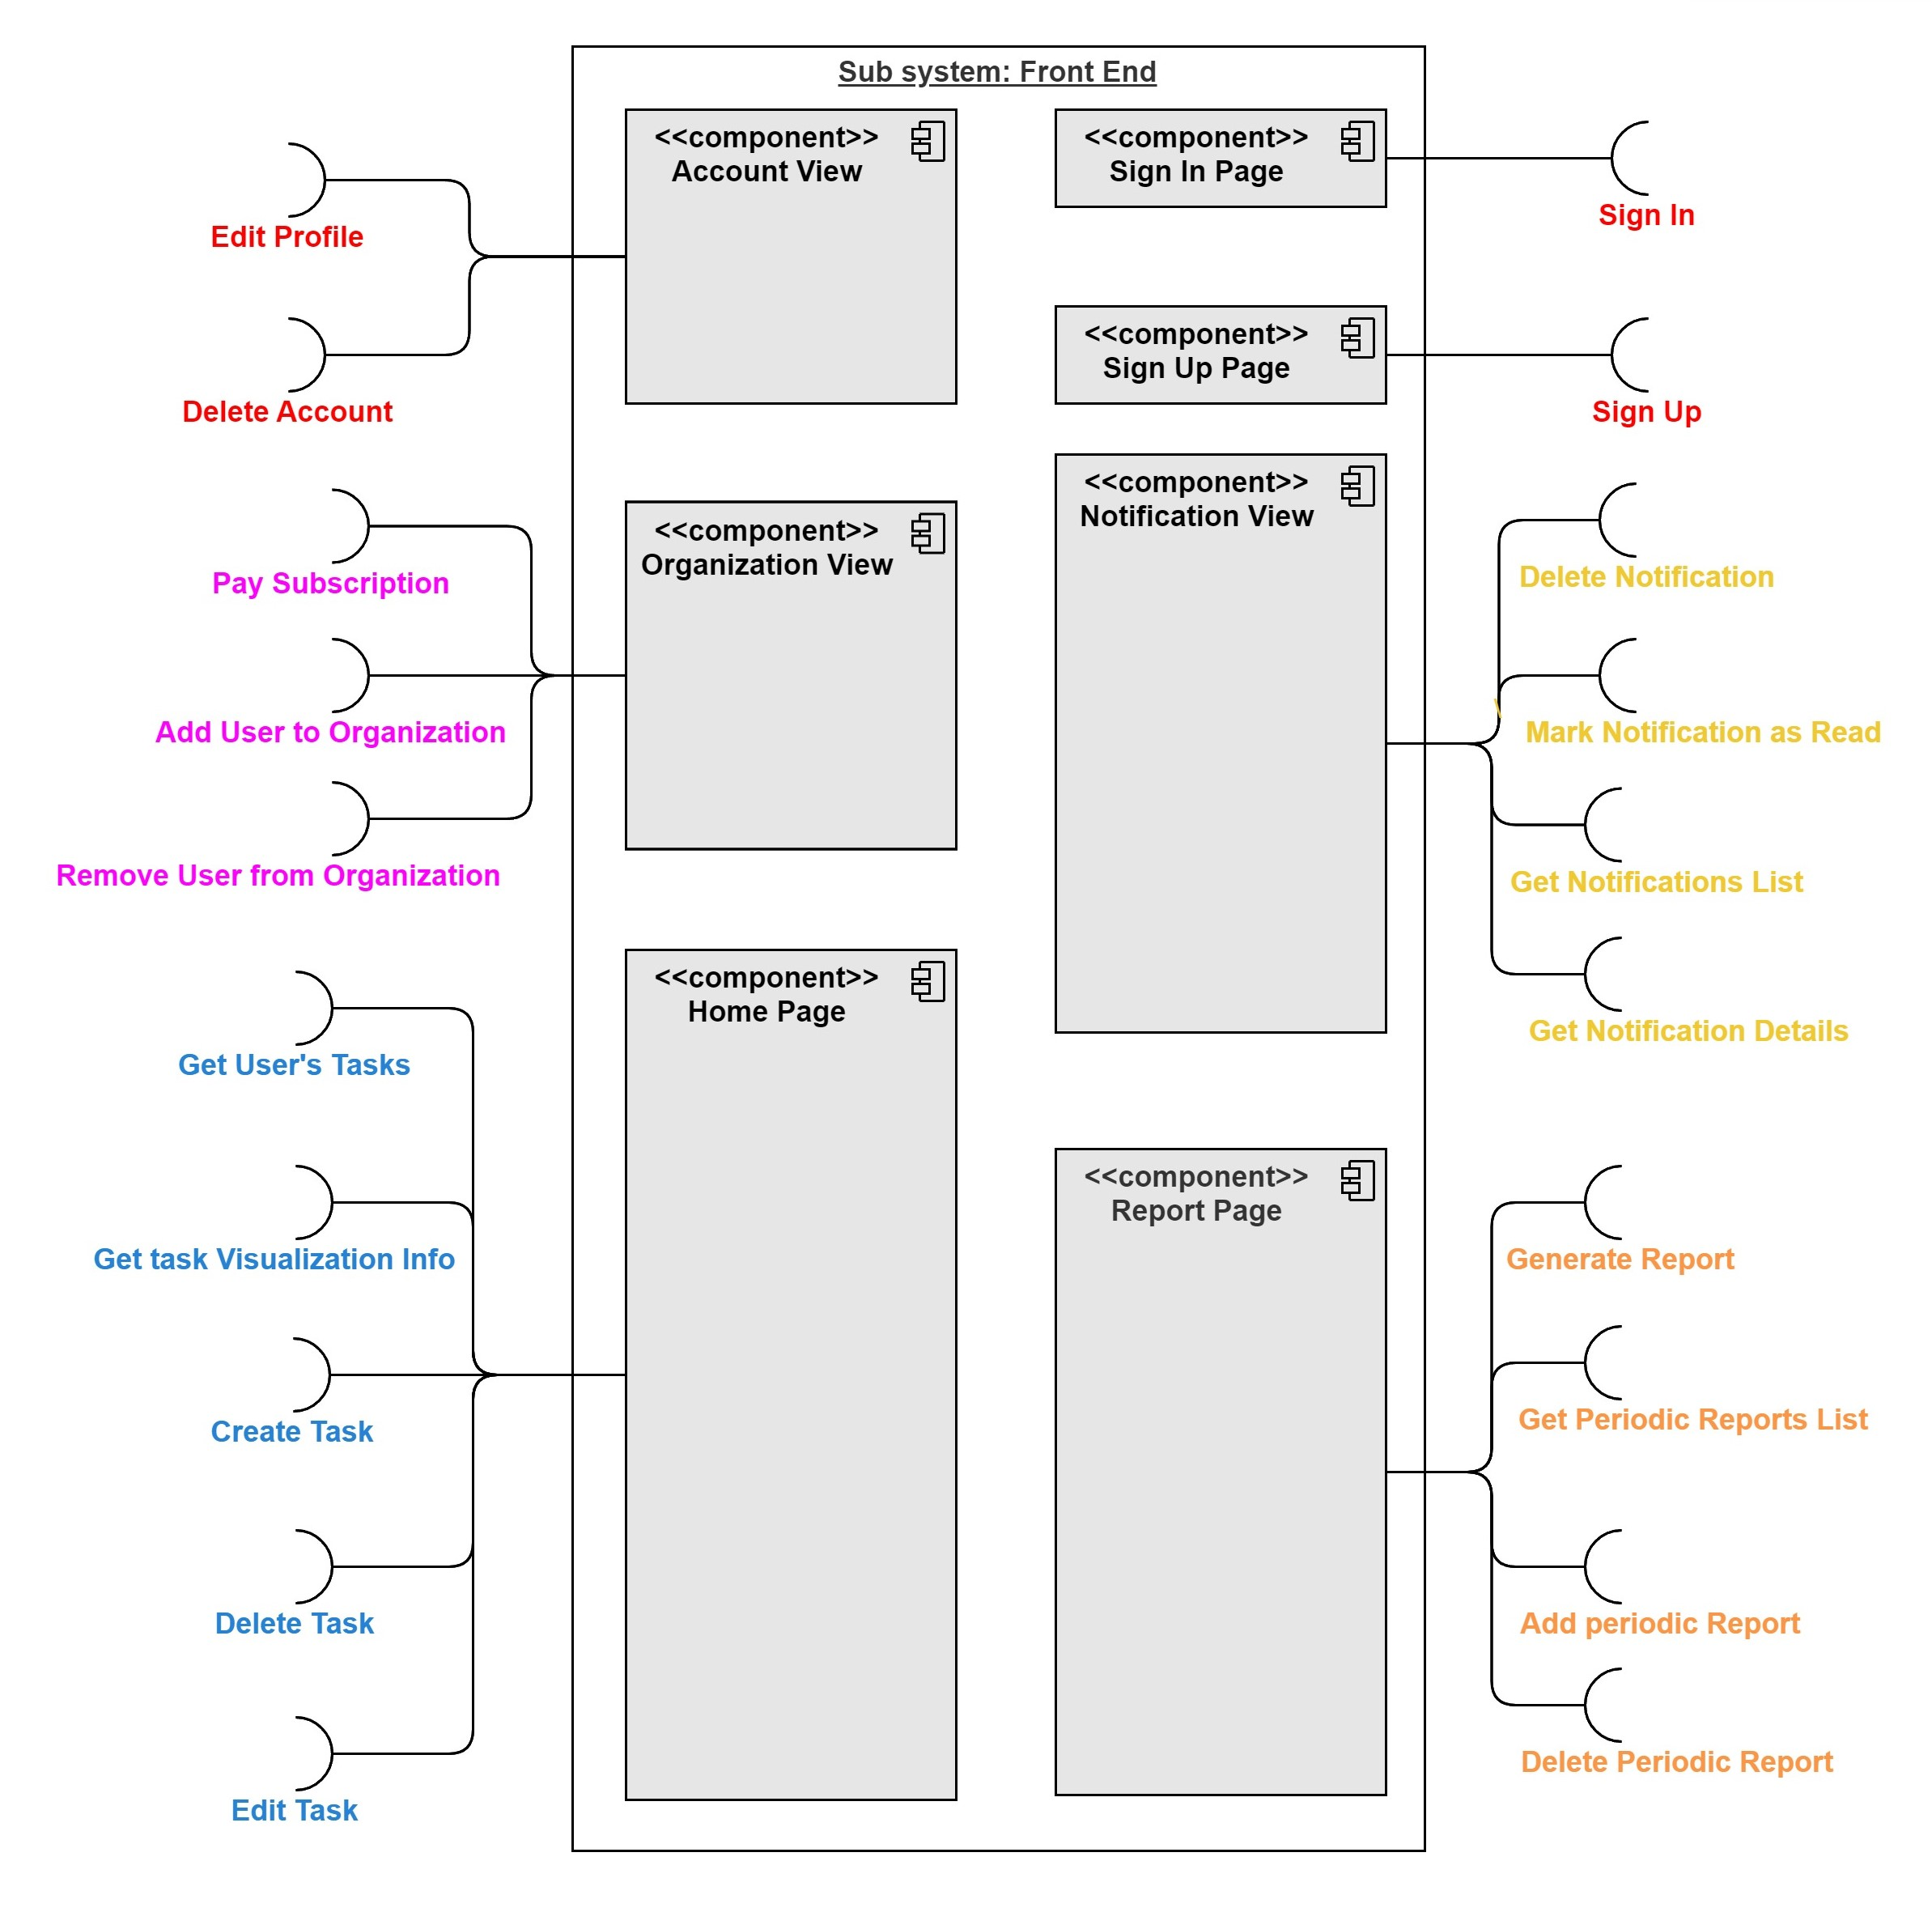
\includegraphics[width=\textwidth,height=\textheight,keepaspectratio]{images/component_diagram/front_end.jpg}
\subsubsection{Descriptions}
In the front end diagram we decided to create one component for every page of the application, for a total of 7 components:
\begin{itemize}
    \item \textbf{Sign In Page: } In this page the users will be able to sign in to the application.
    \item \textbf{Sign Up Page: } In this page the users will be able to sign up for the application
    \item \textbf{Home Page: } This is the main page of the application, where the user will be able to see/edit/create all the tasks of the organization.
    \item \textbf{Report Page: } This page will allow users to ask for a report, or set up a Periodic Report.
    \item \textbf{Notification View: } This page will allow users to see all the pending notifications.
    \item \textbf{Organization View: } This page will allow the organization owner to manage the organization, including things like adding/removing users, or paying the subscription.
    \item \textbf{Account View: } This page will allow the user to manage his account, including things like changing the password, or deleting the account.
\end{itemize}
\end{document}
